\documentclass[12pt,a4paper,oneside]{report}

% Packages nécessaires
\usepackage[utf8]{inputenc}
\usepackage[T1]{fontenc}
\usepackage[french]{babel}
\usepackage{pdfpages}
\usepackage{geometry}
\usepackage{fancyhdr}
\usepackage{graphicx}
\usepackage{amsmath}
\usepackage{amsfonts}
\usepackage{amssymb}
\usepackage{hyperref}
\usepackage{url}
\usepackage{cite}
\usepackage{setspace}
\usepackage{tocloft}
\usepackage{listings}
\usepackage{xcolor}
\usepackage{float}
\usepackage{caption}
\usepackage{subcaption}
\usepackage{array}
\usepackage{longtable}
\usepackage{multirow}
\usepackage{booktabs}
\usepackage{pgfgantt}
\usepackage{tikz}
\usepackage{pdflscape}
\usepackage{titlesec}
\usepackage{enumitem}
\usepackage{pifont}
\usetikzlibrary{positioning,shapes,arrows}
\usepackage{lmodern}
\usepackage{microtype}

% Configuration de la page
\geometry{left=2.5cm,right=2cm,top=2cm,bottom=2cm}
\setlength{\headheight}{15pt}
\setstretch{1.3}

% Configuration des en-têtes et pieds de page
\pagestyle{fancy}
\fancyhf{}
\fancyhead[L]{\leftmark}
\fancyfoot[C]{\thepage}

% Configuration des liens hypertexte
\hypersetup{
    colorlinks=true,
    linkcolor=black,
    filecolor=magenta,      
    urlcolor=blue,
    citecolor=black
}

% Configuration pour les listings de code
\lstset{
    backgroundcolor=\color{gray!10},
    basicstyle=\ttfamily\small,
    breaklines=true,
    captionpos=b,
    commentstyle=\color{green!50!black},
    keywordstyle=\color{blue},
    stringstyle=\color{red},
    numbers=left,
    numberstyle=\tiny\color{gray},
    frame=single,
    tabsize=2
}

\lstdefinelanguage{yaml}{
    keywords={true, false, null},
    keywordstyle=\color{blue}\bfseries,
    basicstyle=\ttfamily,
    sensitive=false,
    comment=[l]{\#},
    commentstyle=\color{purple}\ttfamily,
    stringstyle=\color{red}\ttfamily,
    morestring=[b]',
    morestring=[b]"
}

% Définition des informations du document
\newcommand{\titre}{}
\newcommand{\auteur}{Ghassen Chouchen}
\newcommand{\etablissement}{Iset Sousse}
\newcommand{\organisme}{Billcom Consulting}
\newcommand{\annee}{2025-2026}
\newcommand{\encadrant}{Mr name}

% Formatage des titres
\addto\captionsfrench{%
  \renewcommand\chaptername{Chapitre}%
  \renewcommand\contentsname{Table des matières}%
  \renewcommand\listfigurename{Liste des figures}%
  \renewcommand\listtablename{Liste des tableaux}%
  \renewcommand\bibname{Bibliographie}%
}

\renewcommand{\thesection}{\arabic{section}.}
\renewcommand{\thesubsection}{\thesection\arabic{subsection}}
\renewcommand{\thesubsubsection}{\thesubsection.\arabic{subsubsection}}
\setcounter{secnumdepth}{3}
\setcounter{tocdepth}{3}

\titleformat{\section}[hang]
  {\normalfont\Large\bfseries}{\thesection}{1em}{}
\titleformat{\subsection}[hang]
  {\normalfont\large\bfseries}{\thesubsection}{1em}{}
\titleformat{\subsubsection}[hang]
  {\normalfont\large\bfseries}{\thesubsubsection}{1em}{}
\titleformat{\chapter}[hang]
  {\normalfont\huge\bfseries}
  {\normalfont\LARGE\bfseries Chapitre~\thechapter.\hspace{0.5em}}
  {0pt}{}
\titlespacing*{\chapter}{0pt}{-27pt}{20pt}

\renewcommand{\cftchappresnum}{Chapitre~}
\renewcommand{\cftchapaftersnum}{.~}
\setlength{\cftchapnumwidth}{2.6cm}
\setlength{\cftbeforetoctitleskip}{-1.0em}

\let\oldchapter\chapter
\renewcommand{\chapter}{\clearpage\oldchapter}

\begin{document}

% Numérotation romaine pour les pages préliminaires
\pagenumbering{Roman}

% Page de garde

\includepdf[pages=1]{sections/PageGarde.pdf}

% Dédicace
\input{sections/dedicace}

% Remerciements
\input{sections/remerciements}

% Résumé
\input{sections/resume}

% Abstract
\chapter*{Abstract}
\addcontentsline{toc}{chapter}{Abstract}

% Définir manuellement le mark pour les en-têtes
\markboth{Abstract}{Abstract}

% Garder la numérotation romaine visible
\thispagestyle{plain}



\textbf{Keywords:} 
\newpage

% Table des matières
\tableofcontents
\markboth{Table des matières}{Table des matières}
\newpage

% Liste des figures
\listoffigures
\markboth{Liste des figures}{Liste des figures}
\newpage

% Liste des tableaux
\listoftables
\markboth{Liste des tableaux}{Liste des tableaux}
\newpage

% Liste des sigles et acronymes
\chapter*{Liste des abbréviations}
\addcontentsline{toc}{chapter}{Liste des sigles et acronymes}

% Définir manuellement le mark pour les en-têtes
\markboth{Liste des sigles et acronymes}{Liste des sigles et acronymes}

% Garder la numérotation romaine visible
\thispagestyle{plain}

\begin{tabular}{ll}
\textbf{PoC} & Proof of Concept \\
\textbf{PGSQL} & PostgresSQL: Système de gestion de base de données relationnelle \\
\textbf{Spark} & Apache Spark (moteur de traitement distribué de données) \\
\textbf{SQL} & Structured Query Language \\
\end{tabular}

\newpage


% Passage à la numérotation arabe
\pagenumbering{arabic}
\pagestyle{fancy}
\fancyhf{}
\fancyhead[L]{\leftmark}
\fancyfoot[C]{\thepage}

% Introduction générale
\section*{Introduction générale}
\addcontentsline{toc}{section}{Introduction générale}

\section*{Introduction générale}
\addcontentsline{toc}{section}{Introduction générale}

Dans le domaine de l'ingénierie logicielle contemporaine, la conception et le déploiement d'applications d'entreprise connaissent une mutation technologique profonde. Pendant de nombreuses années, les architectures monolithiques ont constitué le standard pour développer des systèmes d'information complets. Bien que ce modèle de conception centralisé ait fait ses preuves pour des projets de complexité modérée, il montre rapidement ses limites dans les environnements soumis à de fortes contraintes de pérennité : les cycles de déploiement sont lents, la dette technique s'accumule, et une défaillance locale peut entraîner l'indisponibilité totale du système. 

C'est pour répondre à cette rigidité structurelle que le paradigme des microservices s'est imposé, complété par l'émergence incontournable de la culture DevOps. Cette nouvelle approche ne se limite plus à écrire du code ; elle redéfinit l'intégralité du cycle de vie du logiciel en prônant l'automatisation, la containerisation, et l'orchestration dynamique sur le Cloud.

C'est dans ce contexte d'innovation technologique que s'inscrit le présent projet de fin d'études, réalisé au sein de la société Billcom Consulting. L'objectif principal est de concevoir, développer, et automatiser le déploiement d'une plateforme métier orientée microservices (ici appliquée à un cas d'usage de facturation et de gestion). Au-delà de la réingénierie logicielle, l'enjeu majeur de ce projet réside dans la mise en \oe{}uvre d'une chaîne DevSecOps complète : de l'intégration continue jusqu'au déploiement GitOps sur un cluster Kubernetes managé, avec une supervision en temps réel.

Pour structurer ce travail, nous avons adopté la méthodologie agile Scrum, articulée autour de quatre "Releases" majeures. Le présent rapport s'organise ainsi en six chapitres distincts :

Le \textbf{premier chapitre} dresse le cadre général du projet, en présentant l'organisme d'accueil, le contexte technologique, la problématique rencontrée ainsi que la solution proposée et la méthodologie de travail adoptée.

Le \textbf{deuxième chapitre} est consacré à l'analyse et la spécification des besoins. Il identifie les acteurs du système, détaille les fonctionnalités attendues sous forme de cas d'utilisation et présente le \textit{Product Backlog} ainsi que le plan de release.

Le \textbf{troisième chapitre} marque le début de la réalisation (Release 1). Il détaille la conception et le développement de l'ensemble des microservices (gestion des clients, catalogue, abonnements et facturation) et la sécurisation des échanges.

Le \textbf{quatrième chapitre} (Release 2) aborde la mise en place de l'infrastructure logicielle. Il explique la containerisation des applications via Docker et leur déploiement sur les environnements Kubernetes, allant d'un cluster local (Minikube) vers le cloud AWS (Amazon EKS).

Le \textbf{cinquième chapitre} (Release 3) est dédié à l'automatisation. Il décrit la mise en place du pipeline CI/CD avec Jenkins, l'intégration des outils d'analyse de qualité et de sécurité (SonarQube, Trivy), et le déploiement continu via ArgoCD.

Enfin, le \textbf{sixième chapitre} (Release 4) expose la mise en place d'une stack complète de monitoring et de supervision à l'aide de Prometheus et Grafana, garantissant ainsi la fiabilité de la solution en production.

\newpage

\clearpage
\pagestyle{fancy}
\markboth{}{}

% Chapitre 1: Cadre général du stage
\chapter{Cadre général du stage}

\section*{Introduction}
\addcontentsline{toc}{section}{Introduction}


Dans ce chapitre, on va présenter le cadre général de notre project. on va d'abord présenter l'entreprise d'accueil, ensuite on va définir le cadre de ce projet de fin d'études à travers l'analyse de l'existant et la présentation de la problématique ainsi que la solution proposée, et enfin on va détailler la méthodologie de conception adoptée.
\section{Présentation de l'organisme d'accueil}
L'entreprise d'accueil est Billcom Consulting, une société de services et de conseil fondée en 2007, Billcom est spécialisée dans l'accompagnement des opérateurs de télécommunications par l'intégration des solutions BSS dont la gestion de la relation client et de la facturation, ainsi que la migration de données.
Basée en Tunisie, l'entreprise exerce ses activités auprès de clients situés à l'international, notamment en Afrique, au Moyen-Orient et en Europe.

\begin{figure}[H]
    \centering
    
\includegraphics[width=0.223\textwidth]{images/billcom-logo-2.png}
    \caption{Logo de la société d'accueil}
    \label{fig:billcom-logo}
\end{figure}

\begin{table}[H]
    \centering
    \renewcommand{\arraystretch}{1.3}
    \begin{tabular}{|>{\bfseries}l|l|}
        \hline
        Raison sociale & Billcom Consulting \\
        \hline
        Forme juridique & SARL \\
        \hline
        Adresse & Rue des Orangers Hammam Sousse \\
        \hline
        Téléphone & 58597507 \\
        \hline
        E-mail & contact@billcom-consulting.com \\
        \hline
        Secteur d'activité & Conseil et intégration de solutions télécoms \\
        \hline
    \end{tabular}
    \caption{Fiche d'identification de l'entreprise d'accueil}
    \label{tab:organisme_accueil}
\end{table}
\subsection{Services et domaine d'activité}

Afin de mieux présenter le domaine d'activité de Billcom Consulting, on va citer les services et les solutions offerts par cette société :

\begin{itemize}
    \item \textbf{Inégration des solutions de facturation et gestion client :}  déployer et maintenir des systèmes de gestion des abonnés (Customer Care) et des systèmes de facturation, incluant notamment les solutions technologiques de type BSS.

    \item \textbf{Business Consulting :} accompagner les clients dans l'analyse de leurs besoins, l'étude de leurs processus et le choix de solutions techniques et fonctionnelles cohérentes avec leurs objectifs.

    \item \textbf{Support technique :} assurer le support technique, la maintenance des solutions en place et l'assistance aux utilisateurs afin de garantir la continuité de service.

\end{itemize}
\subsection{Clients et collaborateurs}
Billcom Consulting s’est bien positionné sur le marché en fidélisant de nombreux clients. Parmi ceux-ci, on cite :
\begin{figure}[!htbp]
    \centering

\includegraphics[width=\textwidth]{images/clients.png}
\caption{Les clients de Billcom Consulting}
    \label{fig:Les clients de Billcom Consulting}
\end{figure}
\vspace{-0.5cm}
\section{Cadre du projet}
\subsection{Contexte global du projet}
Les opérateurs télécoms s'appuient sur des systèmes d'information complexes pour gérer l'ensemble du cycle de vie de leurs offres et services. Ces systèmes couvrent plusieurs processus métiers essentiels, notamment la gestion des clients, l'abonnement aux offres, le suivi de la consommation, la facturation et le recouvrement.
\newline
\newline
Avec l’évolution des besoins (nombre d’utilisateurs, diversité des offres, intégration avec d’autres systèmes), ces plateformes deviennent de plus en plus complexes à maintenir et à faire évoluer.


\subsection{Étude de l'existant}
Afin de justifier pleinement les choix architecturaux et technologiques opérés dans la création de notre application de gestion des services commercials, il est essentiel d'anlayser les systèmes actuellement utilisés chez les opérateurs télécoms.
\newline

Pour éviter de développer ces systèmes complexes en interne, la majorité des opérateurs se tourne vers des éditeurs logiciels spécialisés proposant des suites BSS prêtes à l'emploi. 
Dans cette approche, l'ensemble des modules décrits précédemment (CRM, Catalogue, Boutiques, Consommation, Facturation, Paiement) est compilé et regroupé au sein d'une seule et même application massive. 
\newline
On cite quelques solutions similaires:
\begin{itemize}
    \item[--] \textbf {Telkoware}
    \item[--] \textbf {Amdocs Kenan }
\end{itemize}
\begin{figure}[H]
    \centering
    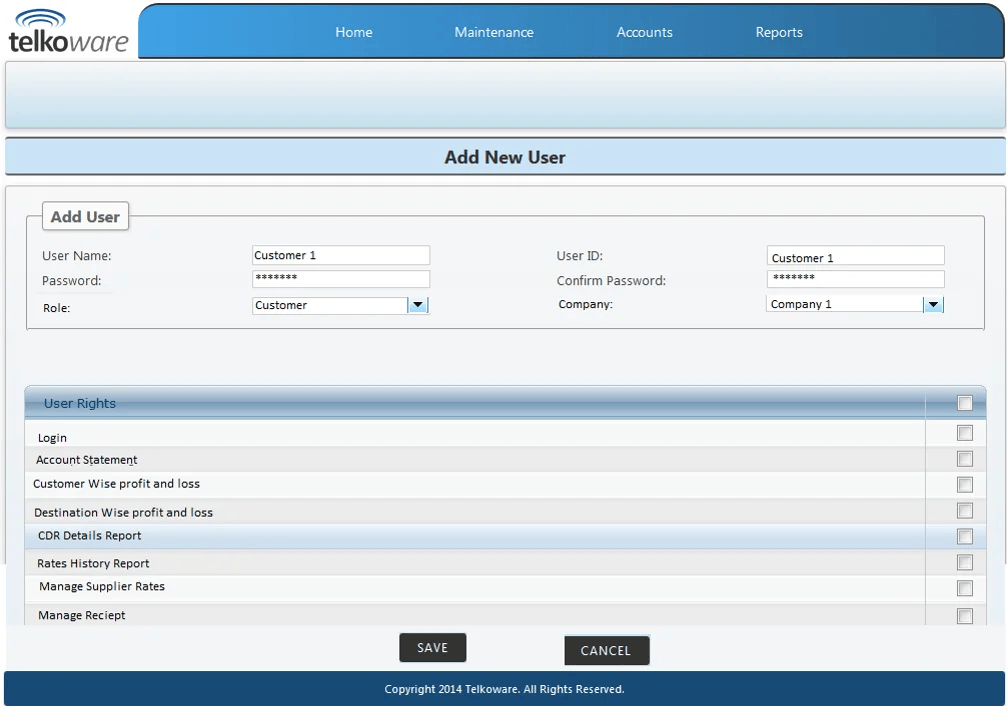
\includegraphics[width=0.9\textwidth]{images/BS-5.png.png}
    \caption{Interface de gestion client de la solution Telkoware}
    \label{fig:Telkoware}
\end{figure}

\subsection{Problématique}
Les équipes informatiques se retrouvent confrontées à plusieurs défis majeurs : la difficulté à livrer de nouvelles fonctionnalités rapidement sans perturber les opérations en cours et la difficulté de faire évoluer un composant du système de manière indépendante
\newline
Ces fonctionnalités sont souvent regroupées au sein de plateformes monolithiques centralisées.
Cette approche visait principalement à simplifier l'intégration initiale et à garantir la cohérence des données entre les différents modules métiers.

\subsection{Solution proposée}
Afin de répondre aux problématiques identifiées, une solution basée sur une architecture modulaire est proposée. Elle s’inspire des systèmes utilisés dans le domaine des télécommunications (BSS), tout en restant adaptée à un contexte de projet de fin d’études.
\newline 
La solution consiste à développer un système organisé en modules indépendants couvrant les principales fonctionnalités métier, notamment la gestion des clients, la gestion des services et des abonnements, la facturation, ainsi que le suivi via un tableau de bord.
Dans ce contexte, on a pensé à des interfaces simples et des actions faciles à utiliser en réduisant la navigation.
\newline
\vspace{-0.5cm}

 Les enjeux de ce projet sont l'automatisation, l'intégration du code ainsi que la livraison continue.
 L'objetif est de mettre en place un pipeline CI/CD, puis le déploiement de l'application dans un cluster Kubernetes, ainsi que l'implémentation d'une partie de surveillance(monitoring) de l'application en environnement de produciton.
 Ce projet s'inscrit dans une démarche DevOps, il constitue quatres phases principales: 
 \begin{itemize}
    \item[•] \textbf{Développment de l'application}
    \item[•] \textbf {Intégration continue / Livraison continue}
    \item[•] \textbf{Déploiement de l'application dans un cluster Kuberentes}
    \item[•] \textbf{Monitoring et alerting}
 \end{itemize}

\section{Langage de modélisation UML}
UML signifie "Unified Modeling Language" ou "Langage de Modélisation Unifié" en français. C'est un langage de modélisation graphique utilisé pour visualiser, spécifier, construire et documenter les systèmes logiciels. UML fournit un ensemble de notations et de diagrammes standardisés qui permettent de présenter le logiciel.
\newline
Il est composé de trois types de diagrammes (diagrammes statiques, diagrammes de comportement et diagrammes dynamiques), chacun ayant une fonction spécifique pour représenter différents aspects du système. Parmi les types de diagrammes les plus couramment utilisés, on trouve : \newline
Les diagrammes de classes, les diagrammes de cas d'utilisation, les diagrammes de séquence et les diagrammes d'activités.

\section{Méthodologie de travail}
Pour mener à bien le développement d'un projet informatique, il est très important de définir la méthode à suivre au cours du travail ainsi que les tâches à effectuer par la suite pour garantir un niveau de qualité acceptable et éviter les délais.

\subsection{Étude comparative des différentes méthodologies}
Le tableau suivant résume les différences entre l'approche classique et l'approche agile.

\begin{table}[H]
    \centering
    \renewcommand{\arraystretch}{1.3}
    \begin{tabular}{|>{\bfseries}p{3cm}|p{5.5cm}|p{5.5cm}|}
        \hline
        Thème & Approche classique & Approche agile \\
        \hline
        Cycle de vie & Séquentiel, en cascade. & Itératif et incrémental. \\
        \hline
        Planification & Définie dès le départ. & Adaptative et évolutive. \\
        \hline
        Documentation & Importante et détaillée. & Réduite au strict nécessaire. \\
        \hline
        Équipe & Rôles spécialisés, pilotage centralisé. & Équipe autonome et collaborative. \\
        \hline
        Changement & Résistance et gestion lourde. & Changement fréquent. \\
        \hline
        Validation & En fin de projet. & Continue, au fil des itérations. \\
        \hline
    \end{tabular}
    \caption{Tableau comparatif entre les méthodologies}
    \label{tab:comparaison_methodologies}
\end{table}
Après une étude comparative des méthodologies , présentées précédemment, nous
avons établi un tableau récapitulatif, illustré par le tableau 1.3 , qui contient les
avantages et les inconvénients de chaque méthode

\vspace{0.3cm}

\begin{table}[H]
    \centering
    \renewcommand{\arraystretch}{1.2}
    \begin{tabular}{|>{\bfseries}p{3.8cm}|p{5.5cm}|p{5.5cm}|}
        \hline
        Méthodologie & Avantages & Inconvénients \\
        \hline
        Classique & {\bfseries - Simple à mettre en oeuvre} \newline {\bfseries - Adaptée aux projets stables} & {\bfseries - Peu flexible} \newline {\bfseries - Spécifications figées dès le départ} \newline {\bfseries - Non adaptable à tout type de projet} \\
        \hline
        Agile & {\bfseries - Livraisons rapides} \newline {\bfseries - Meilleure adaptation aux besoins clients} \newline {\bfseries - Améliore la qualité d'exécution} & {\bfseries - Forte implication requise} \newline {\bfseries - Maîtrise de Scrum nécessaire} \newline {\bfseries - Non adaptable à tout type de projet} \\
        \hline
    \end{tabular}
    \caption{Avantages et inconvénients des méthodologies}
    \label{tab:avantages_inconvenients_methodologies}
\end{table}

\subsection{Choix de méthodologie - Scrum}
La méthode Scrum est une approche agile qu'on a adopté afin de garantir la flexibilité, l'efficacité et l'adaptabilité. Contrairement aux méthodes tradionnelles comme la méthodologie en V ou le modèle en cascade, l'agilité repose sur des cycles courts et itératifs, mieux adaptés aux projets évolutifs.
Elle suppose que le développement d'un logiciel n'est pas prévisibile et ne peut donc pas suivre de processus défini. Ainsi, le résultat du projet n'est pas déterminé au départ, il dépend des retours du client permettant de s'adapter aux imprévus et de maintenir une communication constante avec les parties prenantes.
\newline

La figure suivante présente le schéma décrivant les principes de la méthodologie Scrum. Le principe de base de Scrum est de diviser le projet sur un ensemble d'itérations à réaliser, appelées Sprints. Chaque Sprint possède des buts à atteindre, à partir desquels sont définies les fonctionnalités à implémenter.
Ces fonctionnalités sont définies dans un backlog de produit sous forme de User Stories, qui sont des descriptions courtes et simples d'une fonctionnalité du point de vue de l'utilisateur final.
Un sprint aboutit toujours à la livraison d'une version améliorée et partiellement fonctionnelle du produit appelée MVP.
\begin{figure}[H]
    \centering
    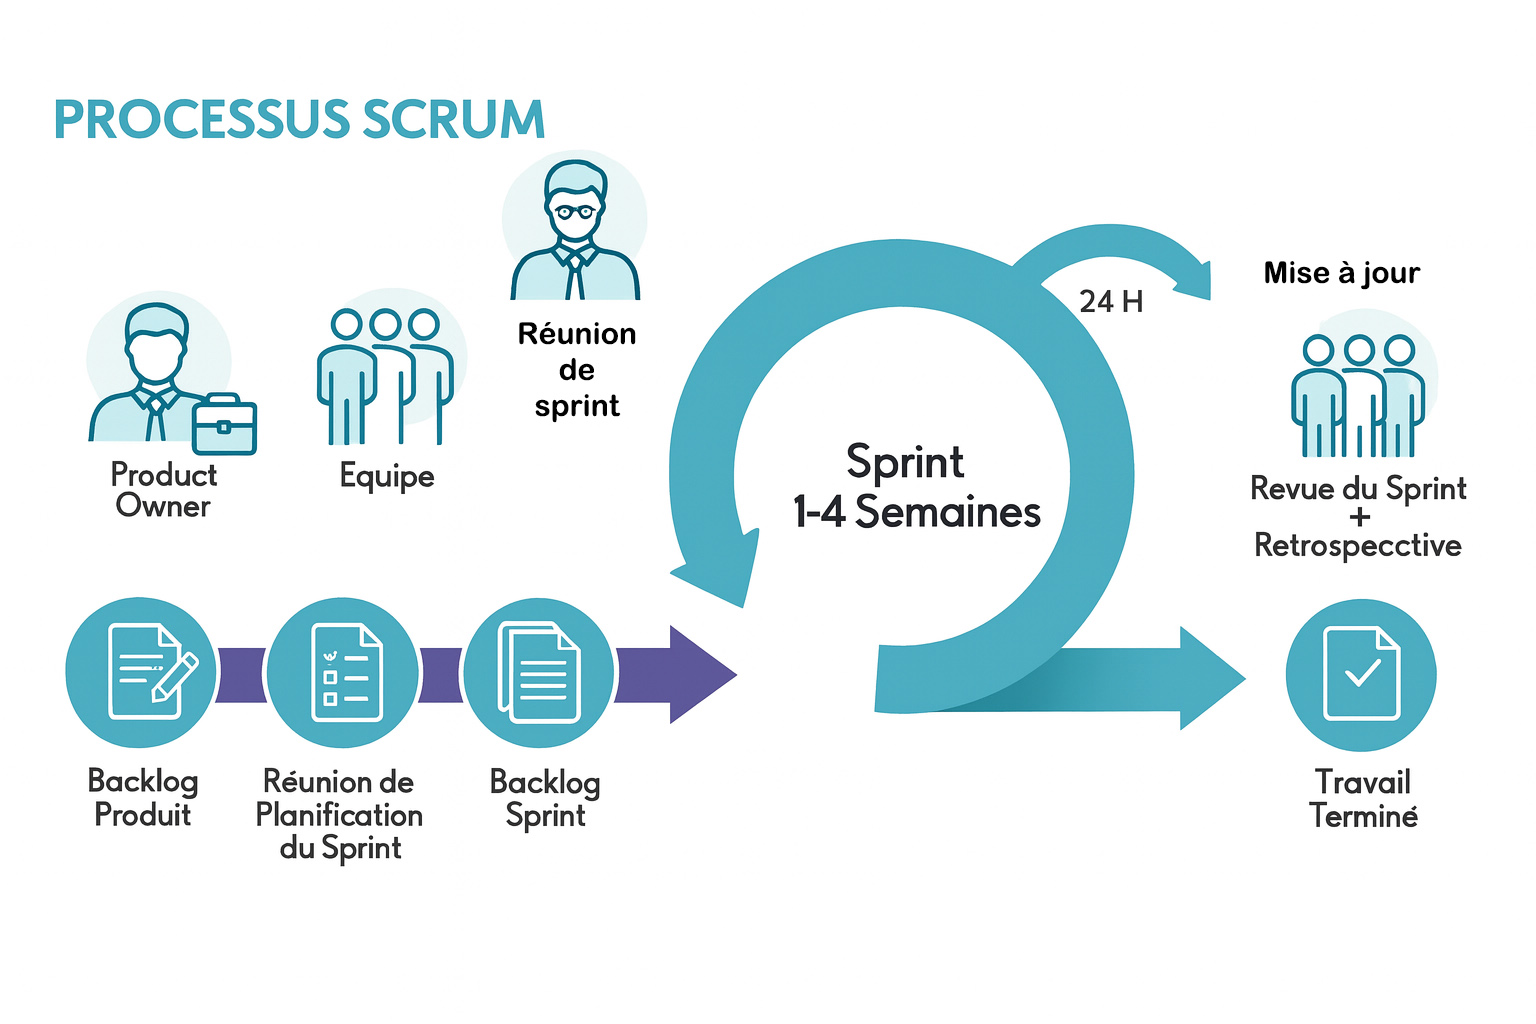
\includegraphics[width=0.8\textwidth]{images/processus-scrum.jpg}
    \caption{La méthodologie Scrum}
    \label{fig:Scrum}
\end{figure}
\subsubsection {Les rôles et les artefacts dans Scrum}
Les trois rôles principaux dans Scrum sont:
 \begin{itemize}
\item[•] \textbf{Product Owner :} il représente le client et les parties prenantes. Il est responsable de maximiser la valeur du produit  il en porte la vision métier. Il définit la feuille de route et gère le \textit{Product Backlog} : contenu, disponibilité et ordre de priorité des éléments.
\vspace{0.16cm}
\newline
\item[•]\textbf{Scrum Master :} il veille au respect du cadre Scrum et facilite son application au quotidien. Son rôle est d'accompagner le Product Owner et l'équipe de développement, de lever les obstacles et de favoriser l'amélioration continue. Ce n'est pas un chef de projet, même si les deux rôles peuvent parfois être cumulés selon le contexte.
\vspace{0.16cm}
\item[•]\textbf{Équipe de développement :} réalise un incrément livrable du produit à chaque Sprint selon les priorités définies. Elle est pluridisciplinaire et peut regrouper différents profils techniques, comme des développeurs, des architectes et des administrateurs de bases de données.
 \end{itemize}
 Les artefacts principaux de Scrum sont:
  \begin{itemize}
\item[•] \textbf{Product Backlog:} Une liste structurée de tous les requis, besoins du client et spécifications du produit. C'est le Product Owner qui est chargé de sa mise à jour tout au long du projet.
\item[•] \textbf{Sprint Backlog:} Un schéma précis des actions à réaliser au cours du Sprint.Il est conçu en début de chaque Sprint à partir du product backlog. Cela permet à l'équipe de surveiller l'avancement et de répondre aux objectifs établis par le Product Owner.
 \end{itemize}
%Maybe include a subsection about the ceremonies
\subsubsection{Justification du choix}
Le choix de la méthodologie Scrum fournit des avantages pour les clients, Scrum permet au client de tester et de valider les fonctionalités au fur et à mesure de leur développement ce qui permet d'obtenir un retour d'information rapide et de s'assurer que le produit final correspond aux attentes du client permettant de minimiser les problèmes de compréhension de la conception. En plus, le client peut ajouter ou modifier les fonctionalités pendant le sprint planning ou le sprint review. Ainsi, Scrum assure la qualité du produit livré.

\section*{Conclusion}
Dans ce chapitre, on a présenté l'entreprise d'accueil, le cadre général de notre projet. Par la suite on a proposé la solution adoptée suite à l'étude de l'existant. Enfin, on a détaillé la méthodologie de travail à suivre pour mener à bien le projet. 

\newpage


% Chapitre 2: Analyse et spécification des besoins
\chapter{Analyse et spécification des besoins}

\section*{Introduction}
\addcontentsline{toc}{section}{Introduction}

L'étape de spécification des besoins constitue la base de départ de ce travail. Ce chapitre comprend l'analyse des besoins fonctionnels et non fonctionnels, l'identification des acteurs, la définition du backlog produit et la planification des releases et des sprints selon la méthodologie Scrum.

\section{Spécification des besoins}

\subsection{Identification des acteurs}

Un acteur représente une entité externe qui interagit avec le système. L'analyse des besoins métier et de l'architecture de l'application a permis d'identifier trois acteurs principaux :

\begin{itemize}
\item[•] \textbf{Administrateur :} Supervise l'ensemble de la plateforme. Il gère les utilisateurs et leurs rôles, administre le catalogue des offres et des services télécom, consulte l'historique de facturation et dispose d'un accès complet à toutes les fonctionnalités du système.

\item[•] \textbf{Agent commercial :} Représente l'utilisateur opérationnel. Il crée et gère les fiches clients, souscrit des abonnements, consulte le catalogue des offres disponibles et effectue les opérations de vente au niveau de la boutique.

\item[•] \textbf{Responsable boutique :} Gère un point de vente. Il administre le stock de cartes SIM, supervise l'équipe commerciale, met à jour les informations des clients rattachés à sa boutique et consulte les abonnements au niveau de son point de vente.
\end{itemize}

\subsection{Besoins fonctionnels}
Les besoins fonctionnels représentent les attentes de chaque acteur vis-à-vis des modules à développer.\newline
Le tableau suivant détaille les besoins fonctionnels identifiés, regroupés par acteur du système :
\newpage
\vspace*{0.75cm}
\renewcommand{\arraystretch}{1.35}

\begin{longtable}{|>{\bfseries}p{4.3cm}|p{11.5cm}|}
    \hline
    \textbf{Acteur} & \textbf{Besoin fonctionnel} \\
    \hline
    \endfirsthead
    \hline
    \textbf{Acteur} & \textbf{Besoin fonctionnel} \\
    \hline
    \endhead
    \hline
    \endfoot
    
    \multirow{6}{*}{Administrateur} 
    & Gérer les utilisateurs et attribuer les rôles. \\ \cline{2-2}
    & Gérer les offres commerciales et les services télécom. \\ \cline{2-2}
    & Consulter l'historique détaillé de facturation des clients. \\ \cline{2-2}
    & Gérer les boutiques. \\ \cline{2-2}
    & Gérer le cycle de vie des abonnements. \\ \cline{2-2}
    \hline
    
    \multirow{6}{*}{Agent commercial}
    & Créer un nouveau client avec validation (CIN, téléphone). \\ \cline{2-2}
    & Consulter et rechercher le profil d'un client. \\ \cline{2-2}
    & Consulter le catalogue des offres disponibles. \\ \cline{2-2}
    & Souscrire un abonnement liant un client à une offre. \\ \cline{2-2}
    & Générer et exporter des factures en PDF. \\ \cline{2-2}
    & Envoyer une facture par email au client. \\ \cline{2-2}
    \hline
    
    \multirow{5}{3cm}{Responsable boutique}
    & Consulter la liste et les détails des boutiques. \\ \cline{2-2}
    & Gérer le stock de cartes SIM (ajout, activation, suspension). \\ \cline{2-2}
    & Gérer l'équipe commerciale de la boutique. \\ \cline{2-2}
    & Mettre à jour les informations des clients rattachés. \\ \cline{2-2}
    & Consulter les abonnements au niveau du point de vente. \\ \cline{2-2}
    \hline
    
    \caption{Besoins fonctionnels par acteur}
    \label{tab:besoins_fonctionnels}
\end{longtable}


\subsection{Besoins non fonctionnels}
Les besoins non fonctionnels définissent les contraintes de qualité, de performance et de sécurité que le système doit respecter.
\begin{itemize}
    \item[•] \textbf{Scalabilité :} Chaque microservice doit pouvoir être mis à l'échelle individuellement en fonction de sa charge, sans impacter les autres services.
    \item[•] \textbf{Disponibilité :} La plateforme doit garantir une haute disponibilité. La défaillance d'un service ne doit pas entraîner l'arrêt du système.
    \item[•] \textbf{Sécurité :} L'accès doit être sécurisé par l'authentification JWT et le contrôle d'accès basé sur les rôles (RBAC). Les mots de passe sont chiffrés.
    \item[•] \textbf{Performance :} Les microservices doivent répondre rapidement aux requêtes, avec des temps de réponse optimisés.
    \item[•] \textbf{Ergonomie :} L'interface doit être intuitive, avec un design minimaliste facilitant la navigation.
\end{itemize}

\section{Diagramme global des cas d'utilisation}

Le diagramme de cas d'utilisation global ci-dessous présente une vue d'ensemble des interactions entre les trois acteurs et les principales fonctionnalités du système.

\begin{figure}[H]
    \centering
    % PLACEHOLDER : Insérer ici le diagramme global des cas d'utilisation
    % Généré à partir du code PlantUML fourni séparément
    % \includegraphics[width=0.95\textwidth]{images/diagramme_cas_utilisation_global.png}
    \fbox{\parbox{0.9\textwidth}{\centering\vspace{3cm}\textbf{[Diagramme global des cas d'utilisation]}\\\vspace{0.2cm}\textit{À générer depuis le code PlantUML fourni}\vspace{3cm}}}
    \caption{Diagramme global des cas d'utilisation}
    \label{fig:use_case_global}
\end{figure}

Les principales interactions sont :
\begin{itemize}
    \item L'\textbf{administrateur} gère le catalogue des services, les offres commerciales et les utilisateurs.
    \item L'\textbf{agent commercial} gère les clients, souscrit des abonnements et traite la facturation.
    \item Le \textbf{responsable boutique} gère le stock de cartes SIM, supervise l'équipe et consulte les données de sa boutique.
\end{itemize}


\section{Planification et priorisation du projet}

\subsection{Pilotage du projet}
Dans le contexte de la méthodologie Scrum, l'équipe se structure autour de trois rôles :

\begin{table}[H]
    \centering
    \renewcommand{\arraystretch}{1.3}
    \begin{tabular}{|>{\bfseries}p{6cm}|p{5cm}|}
        \hline
        \textbf{Rôle} & \textbf{Responsable} \\
        \hline
        Product Owner & Mr. Mohamed Louragini  \\ 
        \hline
        Scrum Master & Mr. Adnen Rouatbi \\ 
        \hline
        Équipe de développement & Ghassen Chouchen \\
        \hline
    \end{tabular}
    \caption{Équipe Scrum du projet}
    \label{tab:pilotage_projet}
\end{table}

\subsection{Technique de priorisation --- MoSCoW}
Le backlog produit est une liste ordonnée de tous les éléments sources de valeur pour le client. Pour assurer une livraison rapide de valeur, il est essentiel de prioriser les éléments du backlog.\newline
Comme technique de priorisation, on a adopté \textbf{la méthode MoSCoW} :
\begin{itemize}
    \item[•] \textbf{M -- Must have :} Éléments essentiels pour le projet.
    \item[•] \textbf{S -- Should have :} Éléments importants mais pas critiques.
    \item[•] \textbf{C -- Could have :} Éléments souhaitables mais non essentiels.
    \item[•] \textbf{W -- Won't have :} Éléments exclus du périmètre actuel.
\end{itemize}

\section{Product Backlog}
Le \textit{backlog produit} regroupe l'ensemble des fonctionnalités à développer, exprimées sous forme de \textit{User Stories} pour les besoins fonctionnels et d'\textit{Enablers} pour les tâches techniques. Ces éléments sont ordonnés et priorisés selon la méthode MoSCoW.

Le tableau~\ref{tab:backlog} présente le backlog produit global du projet.

\renewcommand{\arraystretch}{1.2}
\begin{longtable}{|c|p{2cm}|p{2.2cm}|p{6.8cm}|c|c|}
    \hline
    \textbf{Ordre} & \textbf{Type} & \textbf{Thème} & \textbf{Description} & \textbf{Priorité} & \textbf{Points} \\
    \hline
    \endfirsthead
    \hline
    \textbf{Ordre} & \textbf{Type} & \textbf{Thème} & \textbf{Description} & \textbf{Priorité} & \textbf{Points} \\
    \hline
    \endhead
    \hline
    \endfoot
    
    1 & US & Boutiques & ETQ agent, je veux créer et consulter les boutiques afin de gérer les points de vente. & Must & 5 \\
    \hline
    2 & US & Clients & ETQ agent, je veux créer un client afin de pouvoir lui associer un abonnement. & Must & 8 \\
    \hline
    3 & US & Clients & ETQ agent, je veux modifier un client afin de garder ses informations à jour. & Must & 3 \\
    \hline
    4 & US & Catalogue & ETQ administrateur, je veux gérer le catalogue afin de structurer les services télécom. & Must & 5 \\
    \hline
    5 & US & Offres & ETQ administrateur, je veux créer des offres afin de les proposer aux clients. & Must & 8 \\
    \hline
    6 & US & Abonnements & ETQ agent, je veux souscrire un client à une offre afin de lui fournir un service. & Must & 13 \\
    \hline
    7 & US & SIM & ETQ responsable, je veux gérer le stock SIM afin d'activer les lignes des clients. & Must & 8 \\
    \hline
    8 & US & Auth & ETQ utilisateur, je veux m'authentifier afin d'accéder au système de façon sécurisée. & Must & 5 \\
    \hline
    9 & Enabler & Architecture & Mise en place de l'API Gateway et d'Eureka pour le routage et la découverte des services. & Must & 8 \\
    \hline
    10 & US & Facturation & ETQ agent, je veux générer des factures afin de facturer les abonnements. & Must & 13 \\
    \hline
    11 & US & Facturation & ETQ agent, je veux exporter une facture en PDF afin de la fournir au client. & Must & 5 \\
    \hline
    12 & US & Notification & ETQ agent, je veux envoyer les factures par email afin de notifier le client. & Should & 5 \\
    \hline
    13 & US & Interface & ETQ agent, je veux une interface web afin de gérer facilement les opérations. & Must & 13 \\
    \hline
    14 & Enabler & Déploiement & Création des Dockerfiles et déploiement local des services sur Minikube. & Must & 8 \\
    \hline
    15 & Enabler & Cloud & Provisionnement de l'infrastructure AWS (EKS, RDS, ECR). & Must & 13 \\
    \hline
    16 & Enabler & CI/CD & Mise en place du pipeline Jenkins (build, SonarQube, Trivy, push ECR). & Must & 13 \\
    \hline
    17 & Enabler & GitOps & Configuration d'ArgoCD et Helm pour le déploiement continu. & Must & 8 \\
    \hline
    18 & Enabler & Monitoring & Déploiement de Prometheus et Grafana pour la supervision. & Should & 5 \\
    \hline
    
    \caption{Product Backlog du projet}
    \label{tab:backlog}
\end{longtable}

\textbf{Légende :} US = User Story (besoin fonctionnel), Enabler = Tâche technique.

\section{Plan de release}

Le projet s'étend sur 15 semaines et est organisé en 4 releases contenant au total 7 sprints de 2 semaines chacun, précédés d'une semaine de cadrage et d'analyse.

\begin{table}[H]
    \centering
    \renewcommand{\arraystretch}{1.3}
    \begin{tabular}{|c|p{4cm}|p{8cm}|}
        \hline
        \textbf{Release} & \textbf{Nom du sprint} & \textbf{Objectif} \\
        \hline
        0 & \textit{Cadrage et analyse} & Analyse des besoins et planification \\
        \hline
        1 & Sprint 1, Sprint 2, Sprint 3 &
        \begin{itemize}
            \item Authentification.
            \item Gestion des utilisateurs et des rôles.
            \item Gestion des services métier, des offres et des abonnements.
        \end{itemize} \\
        \hline
        2 & Sprint 4, Sprint 5 &
        \begin{itemize}
            \item Gestion de la containerisation.
            \item Déploiement local sur Minikube.
            \item Déploiement sur AWS avec EKS, RDS et ECR.
        \end{itemize} \\
        \hline
        3 & Sprint 6 &
        \begin{itemize}
            \item Mise en place du pipeline CI Jenkins.
            \item Intégration de SonarQube, Trivy, ArgoCD et Helm.
        \end{itemize} \\
        \hline
        4 & Sprint 7 &
        \begin{itemize}
            \item Mise en place du monitoring.
            \item Déploiement de Prometheus et Grafana.
            \item Création des dashboards de supervision.
        \end{itemize} \\
        \hline
    \end{tabular}
    \caption{Plan de release du projet}
    \label{tab:plan_release}
\end{table}

\section*{Conclusion}
\addcontentsline{toc}{section}{Conclusion}
Dans ce chapitre, nous avons identifié les acteurs du système, spécifié les besoins fonctionnels et non fonctionnels, élaboré le backlog produit priorisé et défini le plan de release. Le chapitre suivant présentera la première release consacrée à la conception et au développement des microservices métier.

\newpage


% Chapitre 3: Release 1 — Conception et développement
\chapter{Release 1 --- Conception et développement}

\section*{Introduction}
\addcontentsline{toc}{section}{Introduction}
Cette release constitue le c\oe{}ur métier de la plateforme de facturation. Elle couvre le développement de l'ensemble des microservices fonctionnels répartis sur trois sprints. Chaque sprint est accompagné de sa modélisation UML (diagrammes de cas d'utilisation, de classes et de séquence).

%======================================================================
% SPRINT 1
%======================================================================
\section{Sprint 1 --- Boutique-service et Customer-service}

\subsection{Objectif du sprint}
Ce sprint vise à mettre en place les deux premiers microservices fondamentaux : la gestion des boutiques (points de vente) et la gestion des clients.

\subsection{Sprint Backlog}

\begin{table}[H]
\centering
\renewcommand{\arraystretch}{1.2}
\begin{tabular}{|c|p{9cm}|c|c|}
\hline
\textbf{ID} & \textbf{Tâche} & \textbf{Priorité} & \textbf{Points} \\
\hline
1.1 & CRUD Boutique (création, consultation, modification) & Must & 5 \\
\hline
1.2 & CRUD Client avec validation CIN (8 chiffres) et téléphone (8 chiffres) & Must & 8 \\
\hline
1.3 & Modification et suspension d'un client & Must & 3 \\
\hline
1.4 & Publication d'événements client via le bus de messages & Should & 3 \\
\hline
\end{tabular}
\caption{Sprint Backlog --- Sprint 1}
\label{tab:sprint1_backlog}
\end{table}

\subsection{Diagramme de cas d'utilisation --- Sprint 1}

\begin{figure}[H]
    \centering
    \fbox{\parbox{0.85\textwidth}{\centering\vspace{2.5cm}\textbf{[Diagramme de cas d'utilisation --- Sprint 1]}\\\vspace{0.2cm}\textit{Gestion des boutiques et gestion des clients}\vspace{2.5cm}}}
    \caption{Diagramme de cas d'utilisation du Sprint 1}
    \label{fig:uc_sprint1}
\end{figure}

\subsection{Diagramme de classes --- Sprint 1}

\subsubsection{Boutique-service}
Le microservice Boutique gère les points de vente et le stock de cartes SIM. Les principales entités sont :
\begin{itemize}
    \item \textbf{Boutique :} Représente un point de vente avec un nom, une adresse, un responsable et un statut (ACTIVE, INACTIVE).
    \item \textbf{SimCard :} Représente une carte SIM avec un numéro ICCID, un statut (AVAILABLE, ASSIGNED, SUSPENDED) et une référence au client assigné.
\end{itemize}

\begin{figure}[H]
    \centering
    \fbox{\parbox{0.85\textwidth}{\centering\vspace{2.5cm}\textbf{[Diagramme de classes --- Boutique-service]}\\\textit{Boutique, SimCard}\vspace{2.5cm}}}
    \caption{Diagramme de classes du Boutique-service}
    \label{fig:class_boutique}
\end{figure}

\subsubsection{Customer-service}
Le microservice Customer gère le cycle de vie des clients. L'entité principale est :
\begin{itemize}
    \item \textbf{Customer :} Contient les informations personnelles du client (nom, prénom, email, CIN, téléphone, adresse), une référence unique (format \texttt{CLT-ANNÉE-UUID}), un statut (ACTIVE, SUSPENDED, TERMINATED) et la référence de la boutique rattachée.
\end{itemize}

\begin{figure}[H]
    \centering
    \fbox{\parbox{0.85\textwidth}{\centering\vspace{2.5cm}\textbf{[Diagramme de classes --- Customer-service]}\\\textit{Customer}\vspace{2.5cm}}}
    \caption{Diagramme de classes du Customer-service}
    \label{fig:class_customer}
\end{figure}

\subsection{Diagramme de séquence --- Créer un client}

\begin{figure}[H]
    \centering
    \fbox{\parbox{0.85\textwidth}{\centering\vspace{2.5cm}\textbf{[Diagramme de séquence --- Créer un client]}\\\textit{Agent commercial $\rightarrow$ API Gateway $\rightarrow$ Customer-service $\rightarrow$ Base de données}\vspace{2.5cm}}}
    \caption{Diagramme de séquence : création d'un client}
    \label{fig:seq_create_customer}
\end{figure}

\subsection{Interfaces réalisées --- Sprint 1}
\begin{figure}[H]
    \centering
    \fbox{\parbox{0.85\textwidth}{\centering\vspace{2.5cm}\textbf{[Capture d'écran --- Liste des boutiques]}\vspace{2.5cm}}}
    \caption{Interface de gestion des boutiques}
    \label{fig:ui_boutiques}
\end{figure}

\begin{figure}[H]
    \centering
    \fbox{\parbox{0.85\textwidth}{\centering\vspace{2.5cm}\textbf{[Capture d'écran --- Liste des clients]}\vspace{2.5cm}}}
    \caption{Interface de gestion des clients}
    \label{fig:ui_clients}
\end{figure}

%======================================================================
% SPRINT 2
%======================================================================
\section{Sprint 2 --- Catalog-service et Subscription-service}

\subsection{Objectif du sprint}
Ce sprint vise à développer le catalogue des services télécom et le mécanisme de souscription aux offres commerciales.

\subsection{Sprint Backlog}

\begin{table}[H]
\centering
\renewcommand{\arraystretch}{1.2}
\begin{tabular}{|c|p{9cm}|c|c|}
\hline
\textbf{ID} & \textbf{Tâche} & \textbf{Priorité} & \textbf{Points} \\
\hline
2.1 & CRUD Service télécom (voix, data, SMS) & Must & 5 \\
\hline
2.2 & CRUD Offre commerciale (regroupement de services) & Must & 8 \\
\hline
2.3 & Souscription d'un client à une offre (création d'abonnement) & Must & 13 \\
\hline
2.4 & Gestion du cycle de vie d'un abonnement (activation, suspension, résiliation) & Must & 5 \\
\hline
\end{tabular}
\caption{Sprint Backlog --- Sprint 2}
\label{tab:sprint2_backlog}
\end{table}

\subsection{Diagramme de cas d'utilisation --- Sprint 2}

\begin{figure}[H]
    \centering
    \fbox{\parbox{0.85\textwidth}{\centering\vspace{2.5cm}\textbf{[Diagramme de cas d'utilisation --- Sprint 2]}\\\textit{Gestion du catalogue et des abonnements}\vspace{2.5cm}}}
    \caption{Diagramme de cas d'utilisation du Sprint 2}
    \label{fig:uc_sprint2}
\end{figure}

\subsection{Diagramme de classes --- Sprint 2}

\subsubsection{Catalog-service}
Le microservice Catalog gère les services télécom et les offres commerciales :
\begin{itemize}
    \item \textbf{ServiceEntity :} Représente un service unitaire (voix, data, SMS) avec un code, un nom, une description et un tarif.
    \item \textbf{Offre :} Regroupe un ensemble de services en une offre commerciale, avec un nom, un prix, une durée de validité et un statut (ACTIVE, DISCONTINUED).
\end{itemize}

\begin{figure}[H]
    \centering
    \fbox{\parbox{0.85\textwidth}{\centering\vspace{2.5cm}\textbf{[Diagramme de classes --- Catalog-service]}\\\textit{ServiceEntity, Offre}\vspace{2.5cm}}}
    \caption{Diagramme de classes du Catalog-service}
    \label{fig:class_catalog}
\end{figure}

\subsubsection{Subscription-service}
Le microservice Subscription gère les abonnements :
\begin{itemize}
    \item \textbf{Abonnement :} Lie un client à une offre avec une date de début, une date de fin, un statut (ACTIVE, SUSPENDED, TERMINATED) et une fréquence de facturation.
\end{itemize}

\begin{figure}[H]
    \centering
    \fbox{\parbox{0.85\textwidth}{\centering\vspace{2.5cm}\textbf{[Diagramme de classes --- Subscription-service]}\\\textit{Abonnement}\vspace{2.5cm}}}
    \caption{Diagramme de classes du Subscription-service}
    \label{fig:class_subscription}
\end{figure}

\subsection{Diagramme de séquence --- Souscrire un abonnement}

\begin{figure}[H]
    \centering
    \fbox{\parbox{0.85\textwidth}{\centering\vspace{2.5cm}\textbf{[Diagramme de séquence --- Souscrire un abonnement]}\\\textit{Agent $\rightarrow$ Gateway $\rightarrow$ Subscription-service $\rightarrow$ Customer-service (Feign) $\rightarrow$ BD}\vspace{2.5cm}}}
    \caption{Diagramme de séquence : souscription d'un abonnement}
    \label{fig:seq_subscribe}
\end{figure}

\subsection{Interfaces réalisées --- Sprint 2}
\begin{figure}[H]
    \centering
    \fbox{\parbox{0.85\textwidth}{\centering\vspace{2.5cm}\textbf{[Capture d'écran --- Catalogue des offres]}\vspace{2.5cm}}}
    \caption{Interface du catalogue des offres}
    \label{fig:ui_catalog}
\end{figure}

%======================================================================
% SPRINT 3
%======================================================================
\section{Sprint 3 --- Billing-service, Auth, API Gateway et Frontend}

\subsection{Objectif du sprint}
Ce sprint finalise le développement métier avec le service de facturation, l'authentification JWT, le gateway centralisé et l'interface Angular.

\subsection{Sprint Backlog}

\begin{table}[H]
\centering
\renewcommand{\arraystretch}{1.2}
\begin{tabular}{|c|p{9cm}|c|c|}
\hline
\textbf{ID} & \textbf{Tâche} & \textbf{Priorité} & \textbf{Points} \\
\hline
3.1 & Génération de factures pour un abonnement & Must & 13 \\
\hline
3.2 & Export de facture en PDF professionnel & Must & 5 \\
\hline
3.3 & Envoi de facture par email via Brevo SMTP & Should & 5 \\
\hline
3.4 & Authentification JWT avec contrôle RBAC & Must & 5 \\
\hline
3.5 & API Gateway avec routage et filtrage JWT & Must & 8 \\
\hline
3.6 & Interface Angular (boutiques, clients, abonnements, factures) & Must & 13 \\
\hline
3.7 & Eureka Server pour la découverte des services & Should & 3 \\
\hline
\end{tabular}
\caption{Sprint Backlog --- Sprint 3}
\label{tab:sprint3_backlog}
\end{table}

\subsection{Diagramme de cas d'utilisation --- Sprint 3}

\begin{figure}[H]
    \centering
    \fbox{\parbox{0.85\textwidth}{\centering\vspace{2.5cm}\textbf{[Diagramme de cas d'utilisation --- Sprint 3]}\\\textit{Facturation, authentification et interface}\vspace{2.5cm}}}
    \caption{Diagramme de cas d'utilisation du Sprint 3}
    \label{fig:uc_sprint3}
\end{figure}

\subsection{Diagramme de classes --- Sprint 3}

\subsubsection{Billing-service}
Le microservice Billing gère le cycle de vie des factures :
\begin{itemize}
    \item \textbf{Facture :} Contient le numéro de facture, la référence client, le montant HT, le taux de TVA (19\%), le montant TTC, le statut (DRAFT, SENT, PAID, OVERDUE, CANCELLED) et les dates d'émission et d'échéance.
    \item \textbf{LigneFacture :} Représente une ligne dans la facture avec la description du service, la quantité, le prix unitaire et le montant.
\end{itemize}

\begin{figure}[H]
    \centering
    \fbox{\parbox{0.85\textwidth}{\centering\vspace{2.5cm}\textbf{[Diagramme de classes --- Billing-service]}\\\textit{Facture, LigneFacture}\vspace{2.5cm}}}
    \caption{Diagramme de classes du Billing-service}
    \label{fig:class_billing}
\end{figure}

\subsubsection{Authentication-service}
Le microservice Authentication gère l'accès sécurisé :
\begin{itemize}
    \item \textbf{User :} Contient le nom d'utilisateur, le mot de passe chiffré, le rôle (ADMIN, RESPONSABLE\_BOUTIQUE, AGENT\_COMMERCIAL) et le statut du compte.
\end{itemize}

\begin{figure}[H]
    \centering
    \fbox{\parbox{0.85\textwidth}{\centering\vspace{2.5cm}\textbf{[Diagramme de classes --- Authentication-service]}\\\textit{User, Role (enum)}\vspace{2.5cm}}}
    \caption{Diagramme de classes de l'Authentication-service}
    \label{fig:class_auth}
\end{figure}

\subsection{Diagramme de séquence --- Générer une facture}

\begin{figure}[H]
    \centering
    \fbox{\parbox{0.85\textwidth}{\centering\vspace{2.5cm}\textbf{[Diagramme de séquence --- Générer une facture]}\\\textit{Agent $\rightarrow$ Gateway $\rightarrow$ Billing-service $\rightarrow$ Subscription (Feign) $\rightarrow$ Customer (Feign) $\rightarrow$ BD}\vspace{2.5cm}}}
    \caption{Diagramme de séquence : génération d'une facture}
    \label{fig:seq_invoice}
\end{figure}

\subsection{Architecture technique de la Release 1}

\begin{figure}[H]
    \centering
    \fbox{\parbox{0.85\textwidth}{\centering\vspace{3cm}\textbf{[Diagramme d'architecture microservices]}\\\textit{Frontend Angular $\rightarrow$ API Gateway $\rightarrow$ Eureka $\rightarrow$ Services métier $\rightarrow$ MySQL}\vspace{3cm}}}
    \caption{Architecture technique des microservices}
    \label{fig:architecture}
\end{figure}

\subsection{Interfaces réalisées --- Sprint 3}

\begin{figure}[H]
    \centering
    \fbox{\parbox{0.85\textwidth}{\centering\vspace{2.5cm}\textbf{[Capture d'écran --- Interface de facturation]}\vspace{2.5cm}}}
    \caption{Interface de gestion des factures}
    \label{fig:ui_billing}
\end{figure}

\begin{figure}[H]
    \centering
    \fbox{\parbox{0.85\textwidth}{\centering\vspace{2.5cm}\textbf{[Capture d'écran --- Page de connexion]}\vspace{2.5cm}}}
    \caption{Interface d'authentification}
    \label{fig:ui_login}
\end{figure}

\section*{Conclusion}
\addcontentsline{toc}{section}{Conclusion}
Au terme de cette release, l'ensemble des microservices métier sont opérationnels : gestion des boutiques, des clients, du catalogue, des abonnements et de la facturation. L'authentification JWT et l'API Gateway assurent la sécurité et le routage centralisé. Le chapitre suivant abordera la mise en place de l'infrastructure de déploiement.

\newpage


% Chapitre 4: Release 2 — Mise en place de l'infrastructure
\chapter{Release 2 --- Mise en place de l'infrastructure}

\section*{Introduction}
\addcontentsline{toc}{section}{Introduction}
Cette release couvre la containerisation des microservices et leur déploiement, d'abord sur un cluster Kubernetes local (Minikube), puis sur l'infrastructure cloud AWS. Elle est répartie sur deux sprints.

%======================================================================
% SPRINT 4
%======================================================================
\section{Sprint 4 --- Containerisation et déploiement local}

\subsection{Objectif du sprint}
Containeriser l'ensemble des microservices avec Docker et valider leur déploiement sur un cluster Kubernetes local avec Minikube.

\subsection{Sprint Backlog}

\begin{table}[H]
\centering
\renewcommand{\arraystretch}{1.2}
\begin{tabular}{|c|p{9cm}|c|c|}
\hline
\textbf{ID} & \textbf{Tâche} & \textbf{Priorité} & \textbf{Points} \\
\hline
4.1 & Rédaction des Dockerfiles multi-étapes pour chaque microservice & Must & 5 \\
\hline
4.2 & Rédaction du fichier docker-compose.yml pour l'environnement local & Must & 5 \\
\hline
4.3 & Rédaction des manifests Kubernetes (Deployment, Service, ConfigMap) & Must & 8 \\
\hline
4.4 & Déploiement et validation sur Minikube & Must & 5 \\
\hline
\end{tabular}
\caption{Sprint Backlog --- Sprint 4}
\label{tab:sprint4_backlog}
\end{table}

\subsection{Containerisation avec Docker}

Chaque microservice dispose d'un Dockerfile multi-étapes qui sépare la phase de compilation (build) de la phase d'exécution (runtime), permettant de réduire la taille de l'image finale.

\begin{lstlisting}[language=bash, caption={Exemple de Dockerfile multi-étapes}, label={lst:dockerfile}]
# Etape 1 : Compilation
FROM maven:3.9-eclipse-temurin-21 AS build
WORKDIR /app
COPY pom.xml .
COPY src ./src
RUN mvn clean package -DskipTests

# Etape 2 : Execution
FROM eclipse-temurin:21-jre-alpine
COPY --from=build /app/target/*.jar app.jar
EXPOSE 8081
ENTRYPOINT ["java", "-jar", "app.jar"]
\end{lstlisting}

\subsection{Orchestration locale avec Docker Compose}
Le fichier \texttt{docker-compose.yml} orchestre l'ensemble des services en environnement de développement local : base de données MySQL, les microservices Spring Boot, l'API Gateway, le frontend Angular et le serveur Eureka.

\subsection{Déploiement sur Minikube}
Minikube fournit un cluster Kubernetes local pour valider les manifests avant le déploiement en production. Les manifests sont organisés en quatre répertoires :
\begin{itemize}
    \item \texttt{infra/} : MySQL (StatefulSet avec PersistentVolumeClaim).
    \item \texttt{config/} : ConfigMap et Secrets pour les variables d'environnement.
    \item \texttt{services/} : Deployments et Services pour chaque microservice.
    \item \texttt{frontend/} : Deployment et Service pour l'application Angular.
\end{itemize}

\begin{figure}[H]
    \centering
    \fbox{\parbox{0.85\textwidth}{\centering\vspace{2.5cm}\textbf{[Capture d'écran --- Pods sur Minikube]}\\\texttt{kubectl get pods -n billing-dev}\vspace{2.5cm}}}
    \caption{Pods déployés sur le cluster Minikube}
    \label{fig:minikube_pods}
\end{figure}

%======================================================================
% SPRINT 5
%======================================================================
\section{Sprint 5 --- Déploiement sur le cloud AWS}

\subsection{Objectif du sprint}
Provisionner l'infrastructure cloud AWS et déployer la plateforme en environnement de production.

\subsection{Sprint Backlog}

\begin{table}[H]
\centering
\renewcommand{\arraystretch}{1.2}
\begin{tabular}{|c|p{9cm}|c|c|}
\hline
\textbf{ID} & \textbf{Tâche} & \textbf{Priorité} & \textbf{Points} \\
\hline
5.1 & Provisionnement du cluster EKS via la console et CLI AWS & Must & 8 \\
\hline
5.2 & Création de l'instance RDS MySQL & Must & 5 \\
\hline
5.3 & Configuration du registre ECR pour les images Docker & Must & 3 \\
\hline
5.4 & Adaptation des manifests K8s pour l'environnement cloud & Must & 5 \\
\hline
5.5 & Premier déploiement sur EKS et validation & Must & 5 \\
\hline
\end{tabular}
\caption{Sprint Backlog --- Sprint 5}
\label{tab:sprint5_backlog}
\end{table}

\subsection{Architecture de l'infrastructure AWS}
L'infrastructure de production repose sur les services managés suivants :
\begin{itemize}
    \item \textbf{Amazon EKS :} Cluster Kubernetes managé pour l'orchestration des conteneurs.
    \item \textbf{Amazon RDS :} Instance MySQL managée pour la persistance des données.
    \item \textbf{Amazon ECR :} Registre privé pour le stockage des images Docker.
    \item \textbf{Amazon EC2 :} Instance hébergeant le serveur Jenkins pour le pipeline CI/CD.
\end{itemize}

\begin{figure}[H]
    \centering
    \fbox{\parbox{0.85\textwidth}{\centering\vspace{3cm}\textbf{[Diagramme d'architecture AWS]}\\\textit{EC2 (Jenkins) $\rightarrow$ ECR $\rightarrow$ EKS $\rightarrow$ RDS}\vspace{3cm}}}
    \caption{Architecture de l'infrastructure AWS}
    \label{fig:aws_architecture}
\end{figure}

\subsection{Provisionnement du cluster EKS}
Le cluster EKS a été provisionné via la console AWS et l'outil \texttt{eksctl}. La configuration inclut la création de groupes de n\oe{}uds (node groups) avec les ressources nécessaires pour l'exécution des microservices.

\subsection{Configuration d'Amazon RDS}
Une instance MySQL 8.0 a été créée sur Amazon RDS. Les bases de données suivantes sont provisionnées :
\texttt{db\_authentication}, \texttt{db\_customer}, \texttt{db\_catalog}, \texttt{db\_subscription}, \texttt{db\_boutique}, \texttt{db\_billing}.

\begin{figure}[H]
    \centering
    \fbox{\parbox{0.85\textwidth}{\centering\vspace{2.5cm}\textbf{[Capture d'écran --- Console AWS EKS]}\vspace{2.5cm}}}
    \caption{Cluster EKS sur la console AWS}
    \label{fig:aws_eks}
\end{figure}

\section*{Conclusion}
\addcontentsline{toc}{section}{Conclusion}
Au terme de cette release, l'infrastructure de déploiement est opérationnelle : les microservices sont containerisés, validés localement sur Minikube, et l'environnement cloud AWS (EKS, RDS, ECR) est provisionné. Le chapitre suivant abordera l'automatisation du pipeline CI/CD.

\newpage


% Chapitre 5: Release 3 — Pipeline CI/CD
\chapter{Release 3 --- Pipeline CI/CD}

\section*{Introduction}
\addcontentsline{toc}{section}{Introduction}
Cette release vise à automatiser l'intégration et la livraison continues du projet. Elle couvre la mise en place du pipeline Jenkins, l'analyse de qualité avec SonarQube, le scan de sécurité avec Trivy, le packaging avec Helm et le déploiement continu avec ArgoCD.

%======================================================================
% SPRINT 6
%======================================================================
\section{Sprint 6 --- Pipeline CI/CD et déploiement continu}

\subsection{Objectif du sprint}
Mettre en place un pipeline d'intégration et de livraison continues complet, depuis le commit du code jusqu'au déploiement automatique sur le cluster EKS.

\subsection{Sprint Backlog}

\begin{table}[H]
\centering
\renewcommand{\arraystretch}{1.2}
\begin{tabular}{|c|p{9cm}|c|c|}
\hline
\textbf{ID} & \textbf{Tâche} & \textbf{Priorité} & \textbf{Points} \\
\hline
6.1 & Configuration du serveur Jenkins (Dockerfile custom) & Must & 5 \\
\hline
6.2 & Pipeline multi-étapes : build Maven, tests unitaires & Must & 8 \\
\hline
6.3 & Intégration SonarQube pour l'analyse de qualité du code & Should & 5 \\
\hline
6.4 & Scan de sécurité des images avec Trivy & Should & 3 \\
\hline
6.5 & Push automatisé des images vers AWS ECR & Must & 5 \\
\hline
6.6 & Configuration d'ArgoCD et Helm pour le déploiement GitOps & Must & 8 \\
\hline
\end{tabular}
\caption{Sprint Backlog --- Sprint 6}
\label{tab:sprint6_backlog}
\end{table}

\subsection{Architecture du pipeline CI/CD}

Le pipeline CI/CD suit un modèle GitOps. Le processus complet se déroule en deux phases :

\begin{enumerate}
    \item \textbf{Intégration continue (CI)} --- gérée par Jenkins :
    \begin{itemize}
        \item Checkout du code source depuis GitHub.
        \item Compilation avec Maven et exécution des tests unitaires.
        \item Analyse de la qualité du code avec SonarQube.
        \item Construction des images Docker.
        \item Scan de sécurité des images avec Trivy.
        \item Push des images vers AWS ECR.
        \item Mise à jour des tags d'images dans le dépôt de configuration GitOps.
    \end{itemize}
    \item \textbf{Livraison continue (CD)} --- gérée par ArgoCD :
    \begin{itemize}
        \item ArgoCD surveille le dépôt \texttt{billing-app-config} (repo GitOps).
        \item Détection automatique des changements de tags d'images.
        \item Synchronisation automatique des manifests Kubernetes sur le cluster EKS.
    \end{itemize}
\end{enumerate}

\begin{figure}[H]
    \centering
    \fbox{\parbox{0.85\textwidth}{\centering\vspace{3cm}\textbf{[Diagramme du pipeline CI/CD]}\\\textit{GitHub $\rightarrow$ Jenkins (Build, Test, Scan, Push) $\rightarrow$ ECR $\rightarrow$ Config Repo $\rightarrow$ ArgoCD $\rightarrow$ EKS}\vspace{3cm}}}
    \caption{Architecture du pipeline CI/CD}
    \label{fig:cicd_pipeline}
\end{figure}

\subsection{Serveur Jenkins}
Le serveur Jenkins est déployé sur une instance EC2 dédiée. Son image Docker est personnalisée pour inclure tous les outils nécessaires :

\begin{lstlisting}[language=bash, caption={Dockerfile Jenkins personnalisé}, label={lst:jenkins_dockerfile}]
FROM jenkins/jenkins:lts
USER root
RUN apt-get update && \
    apt-get install -y docker.io git curl maven && \
    apt-get clean
# Trivy
RUN curl -sfL https://raw.githubusercontent.com/aquasecurity/
    trivy/main/contrib/install.sh | sh -s -- -b /usr/local/bin
# Helm
RUN curl https://raw.githubusercontent.com/helm/helm/
    main/scripts/get-helm-3 | bash
# AWS CLI
RUN curl "https://awscli.amazonaws.com/awscli-exe-
    linux-x86_64.zip" -o "awscliv2.zip" && \
    unzip awscliv2.zip && ./aws/install
\end{lstlisting}

\subsection{Pipeline Jenkinsfile}
Le pipeline est défini dans un fichier \texttt{Jenkinsfile} déclaratif à la racine du projet.

\begin{figure}[H]
    \centering
    \fbox{\parbox{0.85\textwidth}{\centering\vspace{2.5cm}\textbf{[Capture d'écran --- Pipeline Jenkins]}\\\textit{Vue des stages : Checkout $\rightarrow$ Build $\rightarrow$ SonarQube $\rightarrow$ Docker $\rightarrow$ Trivy $\rightarrow$ ECR $\rightarrow$ Update Config}\vspace{2.5cm}}}
    \caption{Pipeline Jenkins avec les différentes étapes}
    \label{fig:jenkins_pipeline}
\end{figure}

\subsection{Analyse de qualité --- SonarQube}
SonarQube est utilisé pour l'analyse statique du code. Il détecte les bugs, les vulnérabilités et les mauvaises pratiques de code (code smells).

\begin{figure}[H]
    \centering
    \fbox{\parbox{0.85\textwidth}{\centering\vspace{2.5cm}\textbf{[Capture d'écran --- Dashboard SonarQube]}\vspace{2.5cm}}}
    \caption{Résultats d'analyse SonarQube}
    \label{fig:sonarqube}
\end{figure}

\subsection{Scan de sécurité --- Trivy}
Trivy est un scanner de vulnérabilités pour les images Docker. Il est exécuté dans le pipeline Jenkins après la construction de chaque image.

\subsection{Déploiement GitOps avec ArgoCD}
ArgoCD surveille le dépôt de configuration \texttt{billing-app-config} et synchronise automatiquement les manifests Kubernetes sur le cluster EKS.

\begin{figure}[H]
    \centering
    \fbox{\parbox{0.85\textwidth}{\centering\vspace{2.5cm}\textbf{[Capture d'écran --- ArgoCD Dashboard]}\\\textit{Applications synchronisées avec leur statut de santé}\vspace{2.5cm}}}
    \caption{Dashboard ArgoCD}
    \label{fig:argocd}
\end{figure}

\subsection{Packaging avec Helm}
Helm est utilisé pour le packaging des déploiements Kubernetes en production. Les Helm charts permettent de paramétrer les déploiements (image tags, replicas, variables d'environnement) via un fichier \texttt{values.yaml}.

\section*{Conclusion}
\addcontentsline{toc}{section}{Conclusion}
Au terme de cette release, le pipeline CI/CD est pleinement opérationnel. Chaque commit déclenche automatiquement la compilation, les tests, l'analyse de qualité, le scan de sécurité et le déploiement sur le cluster EKS via ArgoCD. Le chapitre suivant abordera la mise en place du monitoring.

\newpage


% Chapitre 6: Release 4 — Monitoring et supervision
\chapter{Release 4 --- Monitoring et supervision}

\section*{Introduction}
\addcontentsline{toc}{section}{Introduction}
Cette dernière release met en place la supervision des microservices déployés sur le cluster Kubernetes. L'objectif est de collecter les métriques des services, de les visualiser à travers des tableaux de bord et de configurer des alertes en cas d'anomalie.

%======================================================================
% SPRINT 7
%======================================================================
\section{Sprint 7 --- Prometheus, Grafana et dashboards}

\subsection{Objectif du sprint}
Déployer une stack de monitoring complète sur le cluster EKS pour superviser la santé et les performances des microservices en production.

\subsection{Sprint Backlog}

\begin{table}[H]
\centering
\renewcommand{\arraystretch}{1.2}
\begin{tabular}{|c|p{9cm}|c|c|}
\hline
\textbf{ID} & \textbf{Tâche} & \textbf{Priorité} & \textbf{Points} \\
\hline
7.1 & Déploiement de Prometheus sur le cluster Kubernetes & Should & 3 \\
\hline
7.2 & Déploiement de Grafana et configuration des sources de données & Should & 3 \\
\hline
7.3 & Création des dashboards de supervision des microservices & Should & 5 \\
\hline
7.4 & Configuration des ServiceMonitors pour le scraping des métriques & Should & 3 \\
\hline
\end{tabular}
\caption{Sprint Backlog --- Sprint 7}
\label{tab:sprint7_backlog}
\end{table}

\subsection{Architecture de monitoring}
La stack de monitoring est composée de trois outils complémentaires :
\begin{itemize}
    \item \textbf{Prometheus :} Système de collecte de métriques. Il interroge (scrape) périodiquement les endpoints \texttt{/actuator/prometheus} exposés par chaque microservice Spring Boot.
    \item \textbf{Grafana :} Plateforme de visualisation. Elle se connecte à Prometheus comme source de données et permet de créer des tableaux de bord interactifs.
    \item \textbf{Alertmanager :} Gestionnaire d'alertes. Il reçoit les alertes de Prometheus et les achemine vers les canaux de notification configurés.
\end{itemize}

\begin{figure}[H]
    \centering
    \fbox{\parbox{0.85\textwidth}{\centering\vspace{3cm}\textbf{[Diagramme d'architecture de monitoring]}\\\textit{Microservices (/actuator/prometheus) $\rightarrow$ Prometheus $\rightarrow$ Grafana}\vspace{3cm}}}
    \caption{Architecture de la stack de monitoring}
    \label{fig:monitoring_architecture}
\end{figure}

\subsection{Déploiement de Prometheus}
Prometheus est déployé sur le cluster Kubernetes dans un namespace dédié \texttt{monitoring}. Les \texttt{ServiceMonitor} (ressources personnalisées) sont configurés pour cibler automatiquement les microservices portant le label \texttt{app.kubernetes.io/part-of: billing-platform}.

\subsection{Dashboards Grafana}
Plusieurs tableaux de bord ont été créés pour visualiser les métriques clés :
\begin{itemize}
    \item \textbf{Vue globale :} Nombre de pods actifs, utilisation CPU et mémoire par service.
    \item \textbf{Requêtes HTTP :} Taux de requêtes, temps de réponse (p50, p95, p99) et taux d'erreurs par microservice.
    \item \textbf{JVM :} Utilisation du heap, nombre de threads actifs et activité du garbage collector.
\end{itemize}

\begin{figure}[H]
    \centering
    \fbox{\parbox{0.85\textwidth}{\centering\vspace{2.5cm}\textbf{[Capture d'écran --- Dashboard Grafana]}\\\textit{Vue globale des microservices}\vspace{2.5cm}}}
    \caption{Dashboard Grafana de supervision}
    \label{fig:grafana_dashboard}
\end{figure}

\begin{figure}[H]
    \centering
    \fbox{\parbox{0.85\textwidth}{\centering\vspace{2.5cm}\textbf{[Capture d'écran --- Prometheus Targets]}\\\textit{Liste des endpoints scrapés}\vspace{2.5cm}}}
    \caption{Targets Prometheus}
    \label{fig:prometheus_targets}
\end{figure}

\section*{Conclusion}
\addcontentsline{toc}{section}{Conclusion}
La mise en place de la stack de monitoring complète cette dernière release. L'ensemble de la plateforme de facturation télécom est désormais opérationnelle en production, avec une supervision continue des performance et de la santé des microservices.

\newpage


% Conclusion générale
\newpage
\section*{Conclusion générale et perspectives}
\addcontentsline{toc}{section}{Conclusion générale}

Ce projet de fin d'études a eu pour ambition la refonte architecturale et le déploiement automatisé d'un système de gestion et de facturation télécom (BSS). Face à la rigidité des systèmes monolithiques traditionnels, la solution proposée a permis de démontrer les bénéfices liés à l'adoption d'une architecture orientée microservices, combinée aux pratiques DevOps modernes.

Tout au long de ce projet, nous avons suivi une démarche agile et itérative, structurée en quatre releases majeures, garantissant une évolution maîtrisée du produit :
\begin{itemize}
    \item \textbf{La conception logicielle :} Nous avons scindé les domaines métier en microservices distincts (Customer, Boutique, Catalog, Subscription, Billing et Auth), assurant ainsi l'indépendance du code et des bases de données.
    \item \textbf{L'orchestration et le Cloud :} Le déploiement s'est concrétisé par la containerisation Docker et la mise en place d'une infrastructure robuste sur Amazon EKS, illustrant la maîtrise des écosystèmes Cloud Native.
    \item \textbf{Culture DevOps et automatisation :} La conception d'un pipeline CI/CD complet via Jenkins, intégrant les tests de sécurité (Trivy), d'analyse de code (SonarQube) et le paradigme GitOps (ArgoCD), a démontré notre capacité à automatiser la chaîne de livraison logicielle.
    \item \textbf{Supervision :} Enfin, la mise en place de Prometheus et Grafana a clôturé le cycle de vie du projet en fournissant la visibilité nécessaire pour garantir la stabilité de l'application en production.
\end{itemize}

Ce projet a été riche en défis techniques et en apprentissages. Il nous a permis d'approfondir nos compétences en ingénierie logicielle (Java, Spring Boot, Angular), en architecture distribuée et en administration d'infrastructures cloud et Kubernetes.

\subsection*{Limites et Perspectives}
Bien que la solution réponde aux objectifs initiaux de ce PoC (Proof of Concept), une prise de recul architecturale permet d'identifier certaines limites, représentant autant de perspectives d'amélioration pour une mise en production industrielle :

\begin{enumerate}
    \item \textbf{Couplage temporel (Le "Monolithe Distribué") :} Actuellement, la communication inter-services repose sur des appels synchrones via OpenFeign (HTTP/REST). Ce choix pragmatique crée un couplage fort : si un service échoue, l'appel en cascade échoue également. La solution radicale pour l'avenir sera la transition vers une \textbf{Architecture Orientée Événements (EDA)} utilisant un broker de messages (Apache Kafka), garantissant l'asynchronisme et la haute résilience.
    
    \item \textbf{Cohérence des données (Saga Pattern) :} En l'absence de transactions de bases de données globales, les erreurs partielles peuvent entraîner des incohérences. L'implémentation du patron \textbf{Saga} permettrait d'orchestrer des transactions distribuées via des requêtes de compensation.
    
    \item \textbf{Gestion des performances et latence réseau :} Les multiples appels réseau nécessaires pour la facturation ralentissent le système. La mise en place du pattern \textbf{CQRS} (Command Query Responsibility Segregation) et d'un système de \textbf{Cache distribué} (Redis) pour des données peu volatiles (comme le catalogue d'offres) réduirait considérablement la latence, à condition de maîtriser l'invalidation de cache pour éviter toute erreur de tarification.
\end{enumerate}

En définitive, ce projet de fin d'études constitue une fondation technique extrêmement solide, alignée sur les standards actuels de l'industrie informatique. Les perspectives identifiées prouvent que l'ingénierie logicielle est un processus d'amélioration continue, visant sans cesse à allier résilience opérationnelle et excellence technique.

\newpage


% Bibliographie
\bibliographystyle{plain}
\bibliography{references}

% Webographie
\input{sections/webographie}

\clearpage
\pagestyle{empty}
\markboth{}{}

\end{document}
